\begin{minipage}{0.65\linewidth}
  \begin{mathpar}
    \inferrule[Lat-UA]{}{\kun \lk \kaff}
    \and
    \inferrule[Lat-AL]{}{\kaff \lk \klin}
    \and
    \inferrule[Lat-Level]{\mul \lk \mul' \and n \lk n'}{\mul_n \lk_\Lat \mul'_{n'}}
  \end{mathpar}
\end{minipage}~
\begin{minipage}{0.2\linewidth}
  \centering
  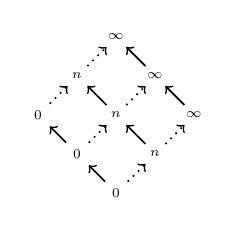
\begin{tikzpicture}
    [->,auto,semithick, every node/.style={scale=0.7}]
    \node(U) {$\kun_0$} ;
    \node(A) [above left of=U] {$\kaff_0$} ;
    \node(L) [above left of=A] {$\klin_0$} ;
    \node(Un) [above right of=U] {$\kun_n$} ;
    \node(An) [above left of=Un] {$\kaff_n$} ;
    \node(Ln) [above left of=An] {$\klin_n$} ;
    \node(Uinf) [above right of=Un] {$\kun_\infty$} ;
    \node(Ainf) [above left of=Uinf] {$\kaff_\infty$} ;
    \node(Linf) [above left of=Ainf] {$\klin_\infty$} ;
    \path
    (U) edge (A)
    (A) edge (L)
    (Un) edge (An)
    (An) edge (Ln)
    (Uinf) edge (Ainf)
    (Ainf) edge (Linf)
    ;
    \path[dotted]
    (U) edge (Un)
    (A) edge (An)
    (L) edge (Ln)
    (Un) edge (Uinf)
    (An) edge (Ainf)
    (Ln) edge (Linf)
    ;
  \end{tikzpicture}
\end{minipage}

%%% Local Variables:
%%% mode: latex
%%% TeX-master: "../main"
%%% End:
